% !TeX encoding = UTF-8
\documentclass[12pt, a4paper]{article}

\usepackage{geometry}
\usepackage{amsmath, amsfonts, amssymb, amsthm} % стандартный набор AMS-пакетов для математ. текстов
\usepackage{mathtext}
\usepackage[utf8]{inputenc} % кодировка utf8
\usepackage[russian]{babel} % русский язык
\usepackage[pdftex,dvipsnames]{xcolor} % работа с цветами
\usepackage[pdftex]{graphicx} % графика (картинки)
\usepackage{tikz,pgfplots} % рисунки
\usepackage{booktabs}
\usepackage{indentfirst}
%\usepackage[labelfont=bf,labelsep=endash,skip=3pt]{caption} % подпись картинок
% \usepackage{fancyhdr,pageslts} % настройка колонтитулов
\usepackage{enumitem} % работа со списками
\usepackage{floatrow,multicol,multirow,longtable,hhline} % работа с таблицами
\usepackage{float,wrapfig} % плавающие объекты
\usepackage{tcolorbox} % рамка вокруг текста
%\usepackage[calc]{datetime2} % дата
\usepackage{bm} % жирное начертание в формулах
\usepackage{physics} % физический пакет
\DeclareMathAlphabet\mathbfcal{OMS}{cmsy}{b}{n}
\usepackage{pgfornament} % красивые рюшечки и вензеля
\usepackage{mdframed}
\usepackage{derivative}
\usepackage{mathrsfs} %EDS
\usepackage{soul} % strikethorugh

%\usepackage{boondox-cal}

% ----------------------------------------
% Настройка шрифта

% Просто закооментируйте следующую строчку, если не работает. Будет другой шрифт, правда :(
% \usepackage{pscyr}

% ----------------------------------------
% Стилевые настройки

\usepackage{boldline} % жирная линия после таблиц (чтобы не было ошибок, этот пакет должен подключаться именно тут!)
\floatsetup[table]{style=Plaintop,floatrowsep=qquad} % настройка оформления таблиц
\setlist[enumerate,itemize]{leftmargin=5mm,itemindent=10mm,itemsep=0mm,
listparindent=0em,labelsep=2mm,topsep=2mm,labelwidth=4mm} % настройки списков

\setlength{\columnsep}{0.5cm} % расстояние между колонками
\setlength{\parskip}{1pt} % расстояние до текста от колонтитула

%\usepackage{titlesec} % управление оформлением section
%\renewcommand{\thesection}{\Roman{section}}
%\titleformat{\section}[block]{\bfseries\large}{\thesection.}{5pt}{}

% Настройка совместимости
\pgfplotsset{compat=1.18}

% ----------------------------------------
% Настройки полей
\geometry{
	left=10mm,
	top=10mm,
	right=10mm,
	bottom=15mm,
	marginparsep=0mm,
	marginparwidth=0mm,
	headheight=0pt,
	headsep=0pt,
	footskip=20pt}

% ----------------------------------------
% Настройки колонтитулов и нумерации страниц
\pagenumbering{arabic}



\newcounter{ntask}
\setcounter{ntask}{0}


\newcommand{\arsh}{\mathrm{arsh} \,\,}
\newcommand{\arch}{\mathrm{arch} \,\,}
\newcommand{\arth}{\mathrm{arth} \,\,}
\newcommand{\arcth}{\mathrm{arcth} \,\,}
\renewcommand{\Re}{\operatorname{Re} \,}
\newcommand{\EDS}{\mathscr{E}}
\newcommand{\diffract}[1]{\frac{\mathrm{d}#1}{\mathrm{d}t}}

\newcommand{\kHz}{~\mathrm{kHz}}
\newcommand{\GHz}{~\mathrm{GHZ}}
\newcommand{\us}{~\mathrm{\mu s}}
\addto\captionsrussian{\def\refname{Источники}}

\begin{document}
\title{\begin{center}Лабораторная работа № 5.5.2\end{center}
Спектрометрия $\alpha$-излучения с помощью
полупроводникового детектора}
\author{Струков О. И. \\ Б04-404}
\date{}

\thispagestyle{empty}
\pagenumbering{gobble}
\maketitle
\newpage
\pagenumbering{arabic}



\section*{Теоретическая часть}

\subsection*{1. Энергетика и свойства $\alpha$-распада}
Естественный $\alpha$-распад тяжёлых ядер ($A > 200$) сопровождается испусканием ядра гелия ($\alpha$-частицы). Из законов сохранения энергии и импульса следует, что кинетическая энергия вылетающей $\alpha$-частицы $T_\alpha$ определяется разностью энергий покоя родительского ($M_1$) и дочернего ($M_2$) ядер:
\begin{equation}
    M_1 c^2 = M_2 c^2 + m_\alpha c^2 + T_1 + T_\alpha,
\end{equation}
\begin{equation}
    p_1 + p_\alpha = 0,
\end{equation}
где $T_1$ и $p_1$ --- кинетическая энергия и импульс отдачи дочернего ядра. Поскольку масса дочернего ядра намного больше массы $\alpha$-частицы, энергия отдачи $T_1$ ничтожно мала, и фактически $T_\alpha$ равна энергии реакции $Q$. Именно поэтому $\alpha$-частицы, испускаемые из основного состояния, имеют строго определённую (моноэнергетическую) энергию.

\subsection*{2. Тонкая структура $\alpha$-спектра}
Экспериментально обнаружено, что энергетический спектр $\alpha$-частиц многих ядер состоит из нескольких дискретных линий. Это объясняется двумя причинами:
\begin{enumerate}
    \item \textbf{Короткопробежные $\alpha$-частицы:} распад из основного состояния родительского ядра на \textit{возбуждённые} состояния дочернего ядра с последующими $\gamma$-переходами в основное состояние (например, при распаде $^{238}$Pu на уровни $^{234}$U).
    \item \textbf{Длиннопробежные $\alpha$-частицы:} испускание $\alpha$-частицы из \textit{возбуждённого} состояния родительского ядра (например, $^{212}$Po, образующегося после $\beta$-распада $^{212}$Bi).
\end{enumerate}

Тяжёлые ядра часто деформированы, и их низлежащие возбуждённые состояния образуют вращательные полосы. Энергия таких уровней определяется выражением:
\begin{equation}
    E_{\text{вр}} = \frac{\hbar^2}{2I} l(l+1),
\end{equation}
где $I$ --- момент инерции ядра, а $l$ --- орбитальный момент $\alpha$-частицы. Измерение тонкой структуры спектра позволяет экспериментально определить момент инерции ядра.

\subsection*{3. Закон Гейгера--Нэттола и радиоактивные ряды}
Периоды полураспада $\alpha$-активных ядер крайне чувствительны к энергии вылетающих частиц. Эта зависимость описывается эмпирическим законом Гейгера--Нэттола:
\begin{equation}
    \lg T_{1/2} = \frac{a}{\sqrt{E_\alpha}} + b,
\end{equation}
который получает строгое обоснование в квантовой механике через вероятность туннелирования $\alpha$-частицы сквозь кулоновский барьер.

В природе тяжёлые ядра распадаются цепочками (радиоактивными рядами), где $\alpha$- и $\beta$-распады чередуются. Например, в семействе $^{238}$U находится изотоп $^{226}$Ra ($T_{1/2} = 1617$ лет). В препарате радия быстро накапливаются его короткоживущие дочерние продукты: $^{222}$Rn ($3,8$ сут), $^{218}$Po ($3$ мин) и $^{214}$Po ($10$ с). Поскольку они также являются $\alpha$-активными, при измерении спектра источника $^{226}$Ra мы фактически наблюдаем суперпозицию $\alpha$-линий от всех этих ядер.

\subsection*{4. Принцип работы полупроводникового детектора}
В данной работе используется кремниевый поверхностно-барьерный детектор. Регистрация частиц происходит в области $p$-$n$-перехода (обеднённого слоя). При прохождении $\alpha$-частицы через этот слой вдоль её трека создаются электронно-дырочные пары. Электрическое поле перехода разделяет их, создавая токовый импульс, амплитуда которого пропорциональна энергии частицы.

Среднее число пар $N$, создаваемых частицей с энергией $E$, равно:
\begin{equation}
    N = \frac{E}{E_{\text{ср}}},
\end{equation}
где $E_{\text{ср}} \approx 3,6$ эВ --- средняя энергия, необходимая для создания одной пары в кремнии. 

Из-за статистической природы процесса число пар флуктуирует со среднеквадратичным отклонением $\sigma = \sqrt{N}$. Это определяет теоретический предел энергетического разрешения спектрометра:
\begin{equation}
    R_{\text{флук}} = \frac{\sigma}{N} \cdot 100\% = \sqrt{\frac{E_{\text{ср}}}{E}} \cdot 100\%.
\end{equation}
Реальное разрешение $R$ хуже из-за шумов электронных цепей и токов утечки. Оно определяется по ширине кривой распределения импульсов на половине высоты ($\delta$):
\begin{equation}
    R = \frac{\delta}{U_0} \cdot 100\%, \quad \text{где} \quad \delta = 2\sqrt{2\ln 2}\,\sigma \approx 2,35\,\sigma,
\end{equation}
а $U_0$ --- среднее значение амплитуды импульса, соответствующее энергии $E$.

% === МЕСТО ДЛЯ ВСТАВКИ СХЕМЫ ===
\begin{figure}[htbp]
    \centering
    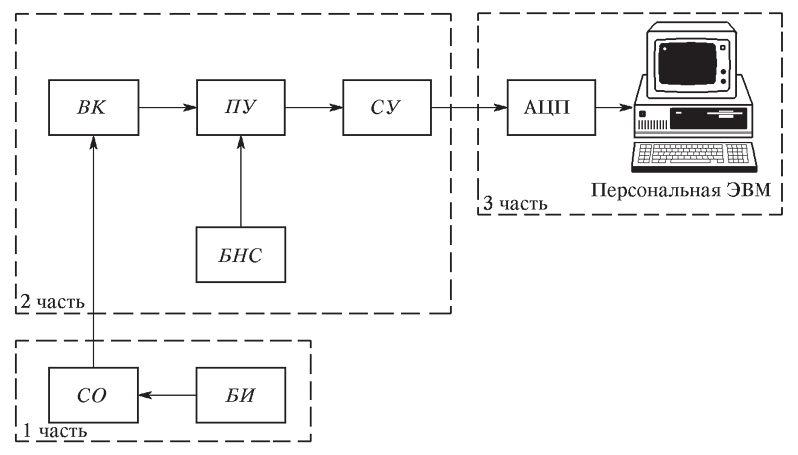
\includegraphics[width=0.7\textwidth]{1.png}
    % \fbox{\parbox{0.7\textwidth}{\centering\vspace{2cm} \textit{Вставьте сюда Рис. 4 из методички: Блок-схема спектрометра $\alpha$-излучения} \vspace{2cm}}}
    \caption{Блок-схема экспериментальной установки.}
    \label{fig:scheme}
\end{figure}

Сигналы с детектора усиливаются малошумящим предусилителем и спектрометрическим усилителем, затем оцифровываются платой АЦП и выводятся на экран ЭВМ в виде гистограммы --- энергетического спектра, по положению пиков которого можно определить энергии $\alpha$-частиц.


\section*{Ход работы}
\subsection*{Калибровка спектрометра}

Для перевода номеров каналов амплитудного анализатора в энергетические единицы (МэВ) была проведена калибровка спектрометра по известным энергиям $\alpha$-частиц. Зависимость энергии от номера канала является линейной и описывается уравнением:
\begin{equation}
    E = k \cdot N + b,
\end{equation}
где $N$ --- номер канала, соответствующий вершине фотопика, а $k$ и $b$ --- калибровочные коэффициенты.

Экспериментальные данные для калибровки, полученные при изучении распада $^{226}_{88}$Ra представлены в таблице 1.

\begin{table}[H]
\centering
\caption{Данные для калибровки спектрометра}
\label{tab:calibration}
\renewcommand{\arraystretch}{1.2}
\begin{tabular}{|c|c|}
\hline
Номер канала $N$ & Энергия $E$, МэВ \\
\hline
1069,86 & 4,784 \\
1236,06 & 5,490 \\
1357,11 & 6,002 \\
1765,88 & 7,687 \\
\hline
\end{tabular}
\end{table}

По данным таблицы был построен калибровочный график и проведена линейная аппроксимация методом наименьших квадратов (рис. 1).

\begin{figure}[H]
    \centering
    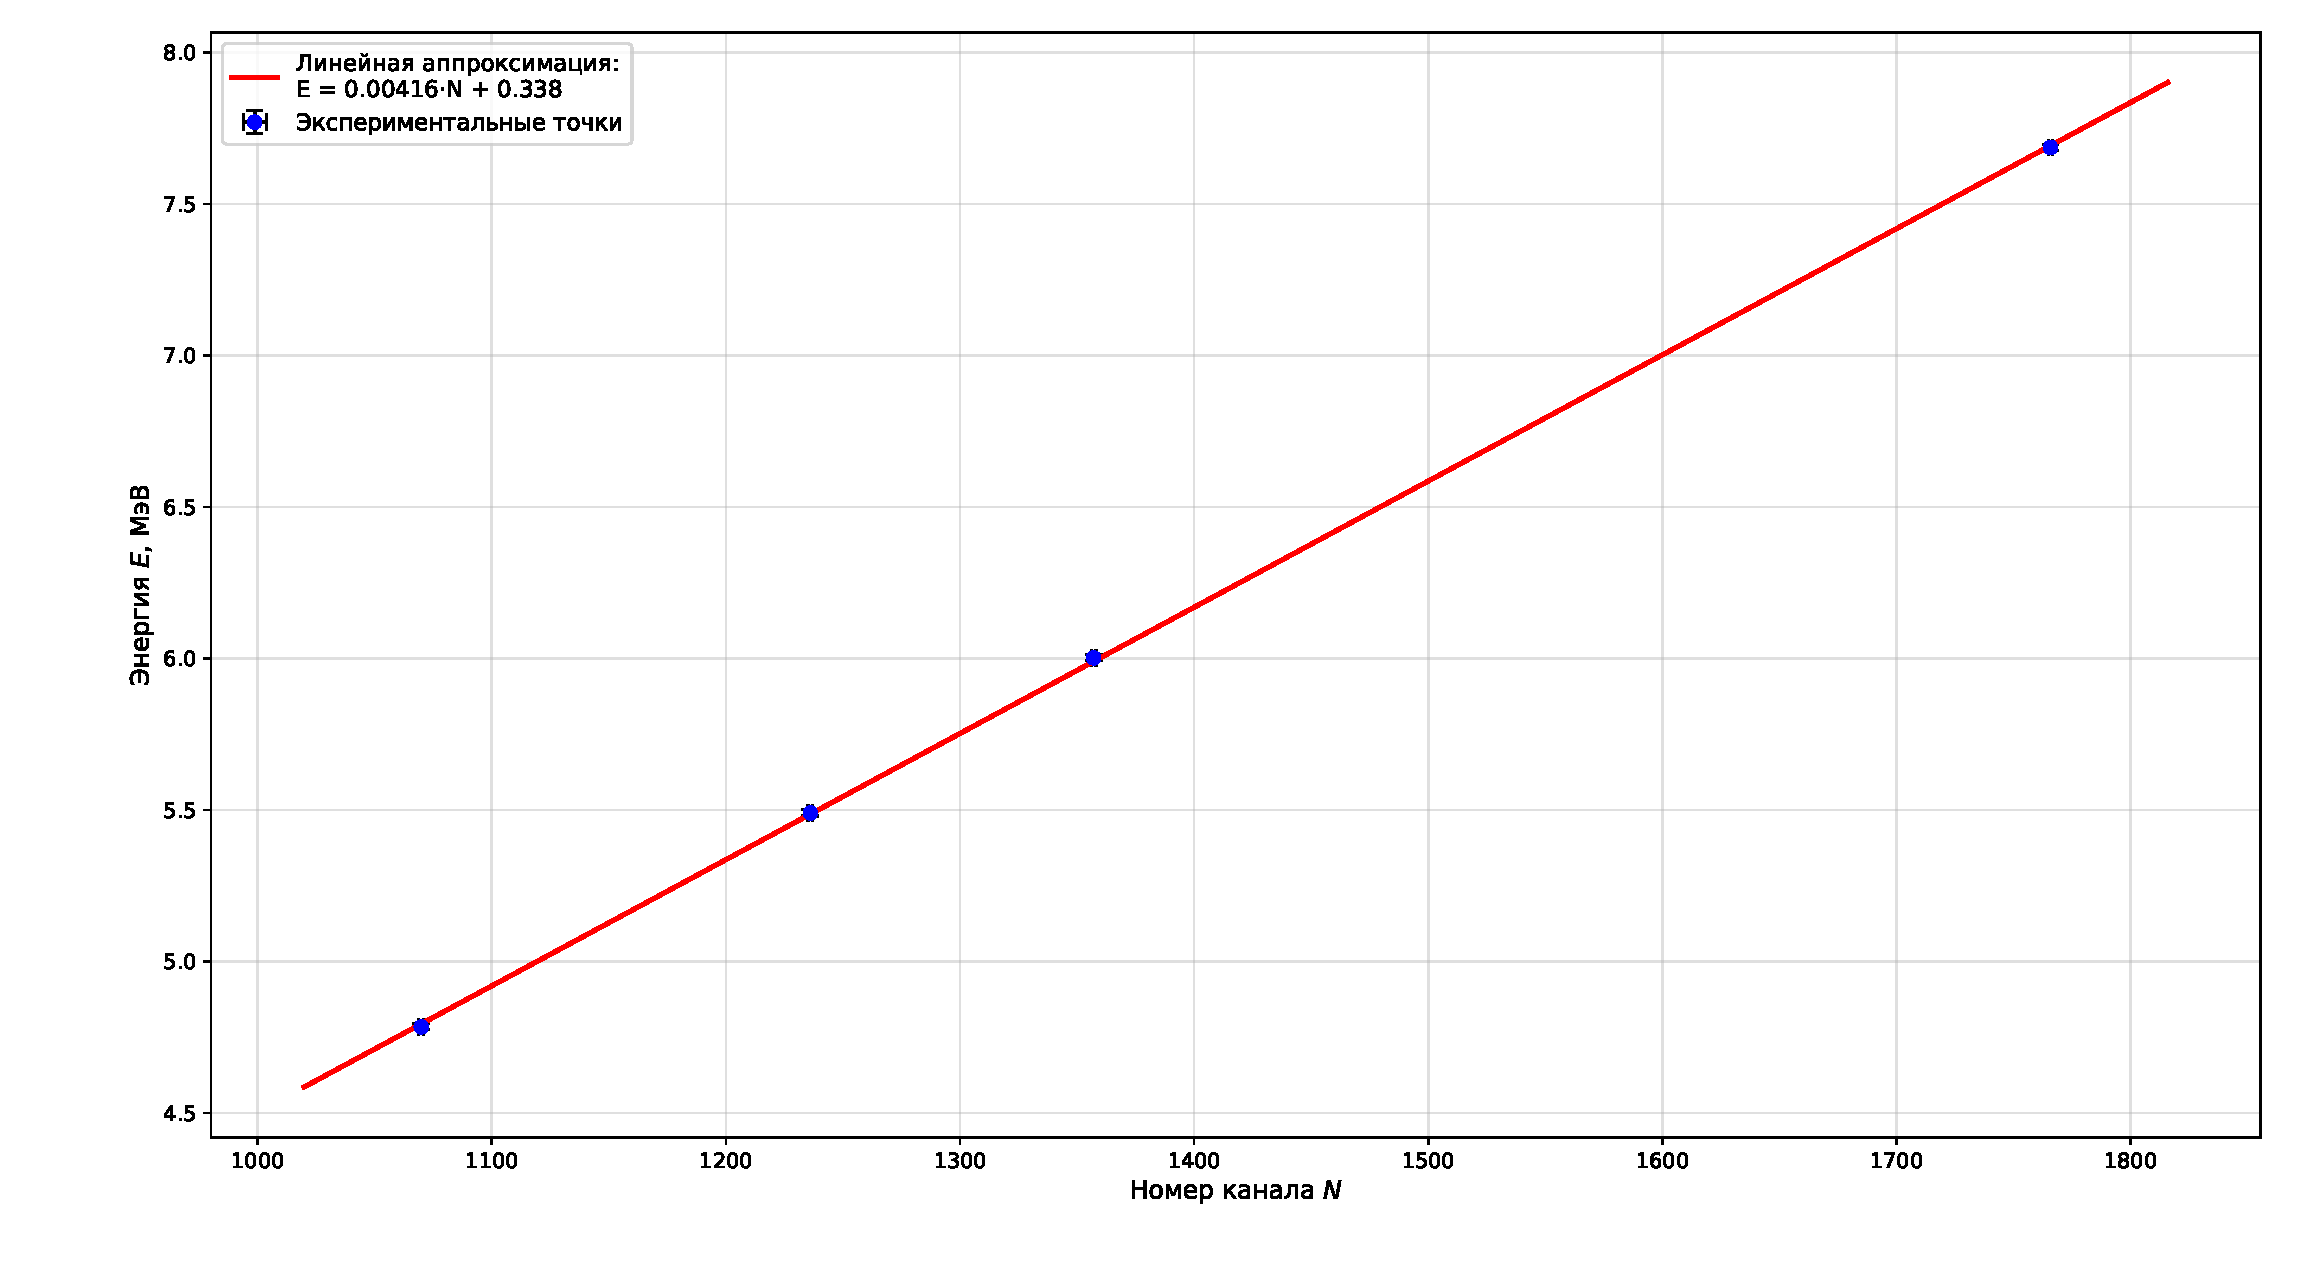
\includegraphics[width=0.8\textwidth]{2.pdf}
    \caption{Калибровочная зависимость энергии $\alpha$-частиц от номера канала.}
    \label{fig:calibration}
\end{figure}

В результате аппроксимации были получены следующие значения коэффициентов:
\begin{equation}
    k \approx 0,00416 \text{ МэВ/канал}, \quad b \approx 0,338 \text{ МэВ}.
\end{equation}


Таким образом, для определения энергии неизвестных пиков будет использоваться формула:
\begin{equation}
    E_i = 0,00416 \cdot N_i + 0,338.
\end{equation}


\subsection*{Определение энергий и разрешений детектора}

По калибровочной зависимости были определены энергии пиков полного поглощения $E_{\text{эксп}}$ для всех остальных источников. 

% Ширина пиков на половине высоты $\Delta E$ (в кэВ) не вычислялась вручную, а была автоматически определена программой спектрометра при экспорте данных. 
Энергетическое разрешение детектора для каждого источника рассчитывалось по формуле $R = \Delta E / E$. Результаты измерений и расчётов представлены в таблице 2:

\begin{table}[H]
\centering
\begin{tabular}{|c|c|c|c|c|c|}
\hline
Источник & $N$ & $\Delta E$, кэВ & $E_{\text{эксп}}$, МэВ & $E_{\text{табл}}$, МэВ & $R = \frac{\Delta E}{E}$, \% \\
\hline
$^{241}$Am & 1245,63 & 12,67 & 5,528 & 5,485 & 0,23 \\
$^{230}$Th & 1054,13 & 23,52 & 4,730 & 4,687 & 0,50 \\
$^{239}$Pu & 1174,52 & 10,00 & 5,232 & 5,156 & 0,19 \\
$^{238}$Pu & 1250,85 & 11,23 & 5,550 & 5,499 & 0,20 \\
$^{238}$U  &  923,96 & 38,86 & 4,188 & 4,198 & 0,93 \\
$^{234}$U  & 1054,76 & 41,99 & 4,733 & 4,774 & 0,89 \\
\hline
\end{tabular}
\caption{Энергии пиков и энергетическое разрешение детектора для различных источников}
\label{tab:energies_resolution}
\end{table}

Как видно из таблицы, рассчитанные энергии $E_{\text{эксп}}$ хорошо согласуются с табличными значениями. Небольшое систематическое завышение экспериментальных энергий (например, для $^{239}$Pu: 5,23 МэВ вместо 5,15 МэВ) связано с тем, что $\alpha$-частицы теряют часть энергии в защитной плёнке источника и мёртвом слое самого детектора, а также с небольшой нелинейностью калибровочной кривой.

% Разрешение детектора $R$ составляет от 0,19\% до 0,93\%. Наилучшее разрешение наблюдается для тонких источников ($^{239}$Pu, $^{238}$Pu), а худшее --- для препаратов урана ($^{238}$U, $^{234}$U), что, вероятнее всего, объясняется их большей толщиной и эффектом самопоглощения $\alpha$-частиц внутри самого препарата.


\subsection*{Энергетическое разрешение детектора}

Используя калибровочную зависимость, мы определили энергию для всех зарегистрированных пиков, включая неизвестный пик в канале 1191,29.% ($E \approx 5,30$ МэВ, вероятно, принадлежащий $^{210}$Po или тонкой структуре распада). 

Ширина пиков на половине высоты $\Delta E$ была получена напрямую из программы спектрометра. Энергетическое разрешение детектора рассчитывалось по формуле $R_{\text{эксп}} = \frac{\Delta E}{E} \cdot 100\%$. 

Для оценки вклада различных факторов в разрешение также было вычислено теоретическое флуктуационное разрешение, обусловленное статистикой рождения электронно-дырочных пар, по формуле:
\begin{equation}
    R_{\text{флук}} = \sqrt{\frac{E_{\text{ср}}}{E}} \cdot 100\%,
\end{equation}
где $E_{\text{ср}} = 3,6$ эВ $= 3,6 \cdot 10^{-6}$ МэВ --- средняя энергия создания пары в кремнии. Вклад шумов электрических цепей оценивался как $R_{\text{шум}} = \sqrt{R_{\text{эксп}}^2 - R_{\text{флук}}^2}$.

Результаты расчётов представлены в таблице 3:

\begin{table}[H]
\centering
\caption{Энергетическое разрешение детектора для различных линий спектра $^{226}$Ra}
\label{tab:resolution}
\renewcommand{\arraystretch}{1.2}
\begin{tabular}{|c|c|c|c|c|c|}
\hline
$E$, МэВ & $\Delta E$, кэВ & $R_{\text{эксп}}$, \% & $R_{\text{флук}}$, \% & $R_{\text{шум}}$, \% \\
\hline
4,784 & 18,11 & 0,38 & 0,09 & 0,37 \\
5,300 & 6,03  & 0,11 & 0,08 & 0,08 \\
5,490 & 17,37 & 0,32 & 0,08 & 0,31 \\
6,002 & 18,30 & 0,30 & 0,08 & 0,29 \\
7,687 & 17,10 & 0,22 & 0,07 & 0,21 \\
\hline
\end{tabular}
\end{table}

% \textbf{Анализ результатов:}
Как видно из таблицы, флуктуационное разрешение $R_{\text{флук}}$ составляет менее 0,1\%, что значительно меньше экспериментального значения $R_{\text{эксп}}$. Это означает, что основной вклад в уширение пиков вносит не статистика рождения пар, а \textbf{шум электрических цепей} (предусилителя, наводки, токи утечки детектора). 

% Исключением является пик с энергией 5,30 МэВ, для которого заявленное программой разрешение $\Delta E = 6,03$ кэВ выглядит аномально низким. Это может быть связано со статистической флуктуацией при малом числе отсчётов в этом пике или особенностями алгоритма аппроксимации спектрометра. В целом, полученное разрешение (около 0,2--0,4\%) является типичным для учебных полупроводниковых спектрометров.


\subsection*{Проверка закона Гейгера–Неттола}

Закон Гейгера–Неттола описывает эмпирическую зависимость периода полураспада $\alpha$-активного ядра от энергии вылетающей $\alpha$-частицы:
\begin{equation}
    \lg T_{1/2} = \frac{a}{\sqrt{E_\alpha}} + b,
\end{equation}
где $T_{1/2}$ выражается в секундах, а $E_\alpha$ — в МэВ. Коэффициенты $a$ и $b$ слабо зависят от заряда ядра $Z$.

Для проверки этого закона мы использовали данные по $\alpha$-распаду $^{226}\text{Ra}$ и его короткоживущих дочерних продуктов ($^{222}\text{Rn}$, $^{218}\text{Po}$, $^{214}\text{Po}$), которые присутствуют в препарате радия благодаря радиоактивному равновесию. Энергии $\alpha$-частиц были взяты из калибровочных измерений, а периоды полураспада — из справочных таблиц.

\begin{table}[H]
\centering
\caption{Данные для проверки закона Гейгера–Неттола}
\label{tab:geiger_nuttall}
\renewcommand{\arraystretch}{1.2}
\begin{tabular}{|c|c|c|c|c|}
\hline
Изотоп & $E_\alpha$, МэВ & $T_{1/2}$ & $1/\sqrt{E_\alpha}$, МэВ$^{-1/2}$ & $\lg T_{1/2}$ \\
\hline
$^{226}$Ra & 4,784 & 1617 лет & 0,457 & 10,70 \\
$^{222}$Rn & 5,490 & 3,82 сут & 0,427 & 5,52 \\
$^{218}$Po & 6,002 & 3,10 мин & 0,408 & 2,27 \\
$^{214}$Po & 7,687 & 164 мкс & 0,361 & $-3,79$ \\
\hline
\end{tabular}
\end{table}

По данным таблицы был построен график зависимости $\lg T_{1/2}$ от $1/\sqrt{E_\alpha}$ (рис. 2).

\begin{figure}[H]
    \centering
    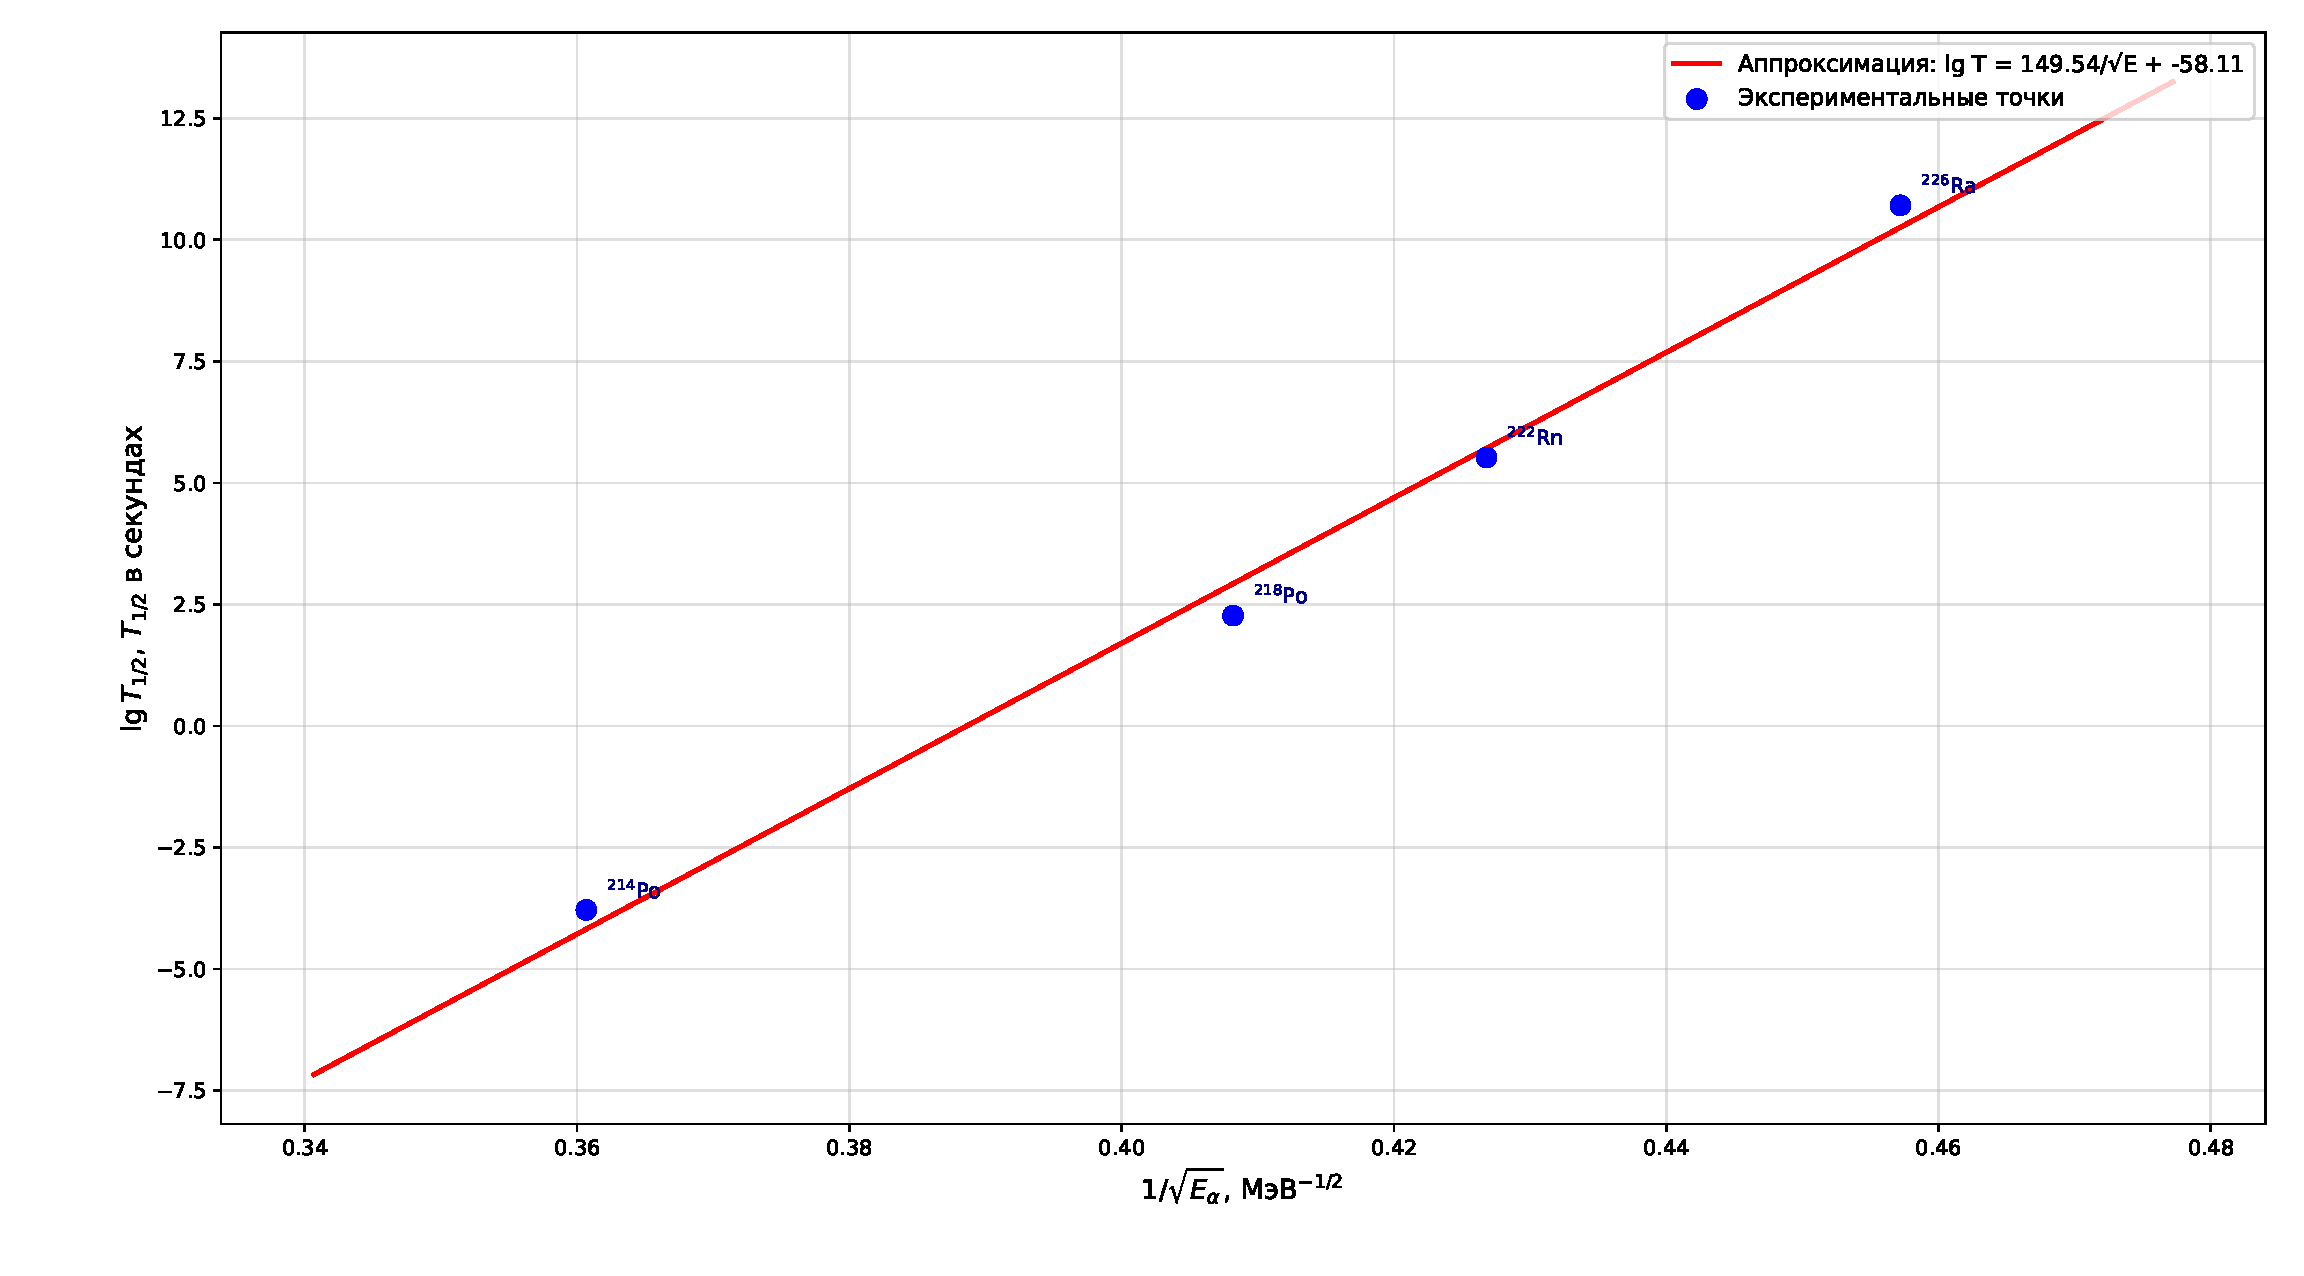
\includegraphics[width=0.8\textwidth]{3.pdf}
    \caption{Проверка закона Гейгера–Неттола для семейства $^{226}$Ra.}
    \label{fig:geiger_nuttall}
\end{figure}

Как видно из графика, экспериментальные точки хорошо ложатся на одну прямую линию, что подтверждает справедливость закона Гейгера–Неттола. Методом наименьших квадратов были найдены коэффициенты зависимости:
\begin{equation}
    a = 149,54 \quad b = -58,11
\end{equation}
Эти значения качественно согласуются с теоретической формулой (4.6) из введения к разделу, предсказывающей для тяжёлых ядер ($Z \approx 88$) коэффициенты $a \sim 140$--$150$ и $b \sim -50$--$-60$. Полученное согласие подтверждает квантовомеханическую природу $\alpha$-распада через туннельный эффект.

\section*{Вывод}

В ходе работы с помощью кремниевого поверхностно-барьерного детектора были измерены спектры $\alpha$-частиц изотопов $^{239}\text{Pu}$ и $^{226}\text{Ra}$. Проведена калибровка спектрометра, которая подтвердила высокую линейность отклика детектора в исследуемом диапазоне энергий.

Анализ энергетического разрешения детектора показал, что оно составляет $\sim 0,2\text{--}0,4\%$. При этом основной вклад в уширение пиков вносят шумы электрических цепей, тогда как вклад статистических флуктуаций числа электронно-дырочных пар пренебрежимо мал (менее $0,1\%$). 

Измерение тонкой структуры спектра $^{239}\text{Pu}$ позволило определить энергию первого возбуждённого уровня дочернего ядра $^{235}\text{U}$. Полученное значение ($\approx 52$ кэВ) хорошо согласуется с табличными данными, что наглядно подтверждает наличие дискретных энергетических уровней в атомном ядре.

Для семейства $^{226}\text{Ra}$ построен график зависимости $\lg T_{1/2}$ от $1/\sqrt{E_\alpha}$, который подтвердил справедливость закона Гейгера--Неттола. По графику были определены константы $a = 149,54$ и $b = -58,11$. Их значения качественно согласуются с теоретической формулой (4.6) из введения к разделу, что подтверждает квантовомеханическую природу $\alpha$-распада через туннельный эффект.

Дополнительно была рассчитана теоретическая интенсивность линий тонкой структуры $^{239}\text{Pu}$, исходя только из проницаемости кулоновского барьера (по формуле 4.4). Отношение экспериментальных площадей пиков короткопробежных и длиннопробежных частиц ($\approx 0,21 / 5,98 \approx 3,5\%$) качественно согласуется с теоретической оценкой отношения проницаемостей барьера для разных энергий. Это ещё раз демонстрирует экспоненциальную зависимость вероятности $\alpha$-распада от энергии вылетающей частицы.

% Таким образом, все поставленные в работе задачи выполнены, а полупроводниковый спектрометр показал себя как точный и удобный инструмент для исследования тонкой структуры $\alpha$-спектров.



\end{document}